\chapter{Conclusions}
\label{cha:conclusion}

This chapter will summarize the main findings of the project.

\section{Stop detection algorithm}

In the final implementation (\autoref{cha:stopdet_impl}), the following parameters were used:

\begin{itemize}  
\item durationsSlidingWindowSize - 1800 s
\item mobilityIndexThreshold - 0.0017 1/s
\item distanceThreshold - 1000 m
\item speedThreshold - 1.4 m/s
\end{itemize}

\begin{figure}[!ht]
	\centering
	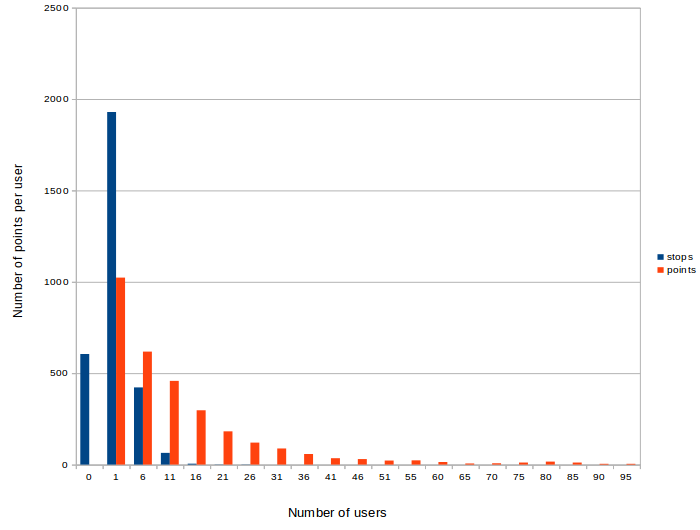
\includegraphics[width=0.8\textwidth]{images/users_count.png}\\
	\caption{ Histogram of number of users having corresponding number of detected stops in the area of Berlin }
	\label{fig:histogram_stops}
\end{figure}

\FloatBarrier

\autoref{fig:histogram_stops} shows, that distribution of recorded points per user follows heavy tailed distribution, and most of the users produced between 1-10 points during the observation period of 24h, within the Berlin area (52.0102, 11.2830, 53.0214, 13.9389). The stop detection algorithm implementation (\autoref{cha:stopdet_impl}) has been able to identify 9022 stops for 2422 unique users, whereas 605 users had no stop at all. \autoref{fig:histogram_stops} additionally shows, that most of the users had between 1-6 stops, and characteristic is also heavy-tailed. 

\begin{table}[ht!]
	\centering
	\caption{Comparison of two analyzed stop detection algorithms for proactive localization}
	\label{tab:alg_comp_table}
	\begin{tabular}{|L|L|L|}
		\hline
		\textbf{Case} & \textbf{Mobility Index} & \textbf{Speed/Distance} 
		\\\hline
		Multiple, slow movements over small area or distance & Possible, but adjusted parameters will cause results to be erroneous for different detections & Very good
		\\\hline
		Single record over small area & Good, but only for longer stays & Very good  
		\\\hline
		Single record over big area & Very good, but only in case of adjusted parameters which might be erroneous at short distances & Possible, but might be erroneous and stops might be mislead with travel due to high speed averages in these cases
		\\\hline
	\end{tabular}
\end{table}

\FloatBarrier

\autoref{tab:alg_comp_table} shows comparison of two approaches to stop detection evaluated in \autoref{cha:eval_stopdetc}. It occurs, that for short distances it is more efficient to use speed/distance algorithm to be able not only capture longer stays at short distance, but also very slow movements in the limited area. For longer distances it is preferable to use mobility index to be able distinguishing travels from stops better using mobility index, which preserves mobility history in the time/duration context for the certain past time window. Using duration based mobility index approach for longer distances allows better stop detection than possibly erroneous speed averaging approach.

\section{Clustering of detected stops}
In this project we used the technique of clustering for detecting popular stop areas. We found that using the density-based clustering algorithm DBSCAN worked well. To be able to run the algorithm for big data, we extended a distributed and parallel DBSCAN implementation on Spark based on MapReduce, called \textit{DBSCAN on spark}. 

Our data was generated from all over Germany, but we started off focusing on the Berlin area. Running the clustering of stop detection gave us clusters in expected places, such as metro stations and plazas. More points where captured at popular "stop points", such as Alexanderplatz (popular plaza and train stop), and Hauphbahnhof (main train station). 

However, we found out that since DBSCAN is highly parameter sensitive, a configuration for a specific area might not give satisfying results for another less, or more, dense area. Running with the parameters on inner Berlin as outer Berlin and rest of Germany yielded few or no clusters (due to less points in close proximity to each other).

To address this we implemented and analyzed an "area version" of DBSCAN on spark. The implementation ran multiple parallel iterations of \textit{DBSCAN on Spark}, each on a specified area of various density with different \textit{epsilon} and \textit{minPts} parameters, and finally merging the results. This addressed our problems of not finding sufficient amount of clusters in less dense areas, which was proven by visualizing our findings in the tool QGIS, along with plotting graphs and histograms. 

We conclude that the best parameters we got for our DBSCAN implementation were:

	\begin{tabular}{|L|L|L|}
		\hline
		\textbf{DBSCAN area version} & \textbf{eps} & \textbf{minPts} 
		\\\hline
		1  & 0.001  & 5
		\\\hline
		2  & 0.003  & 5  
		\\\hline
		3  & 0.005  & 5
		\\\hline
	\end{tabular}

The reason for running with the same \textit{minPts} parameters with bigger \textit{eps} were lack of data points in lesser dense areas, resulting in the need of higher \textit{eps} but not \textit{minPts} for larger areas. Important to remember is that the parameter choice depends on the granuality and application, if we are interested in capturing smaller areas, such as U-bahn/S-bahn stops, we need different parameters than clustering bigger areas, such as big plazas or towns.

\begin{figure}[!ht]
	\centering
	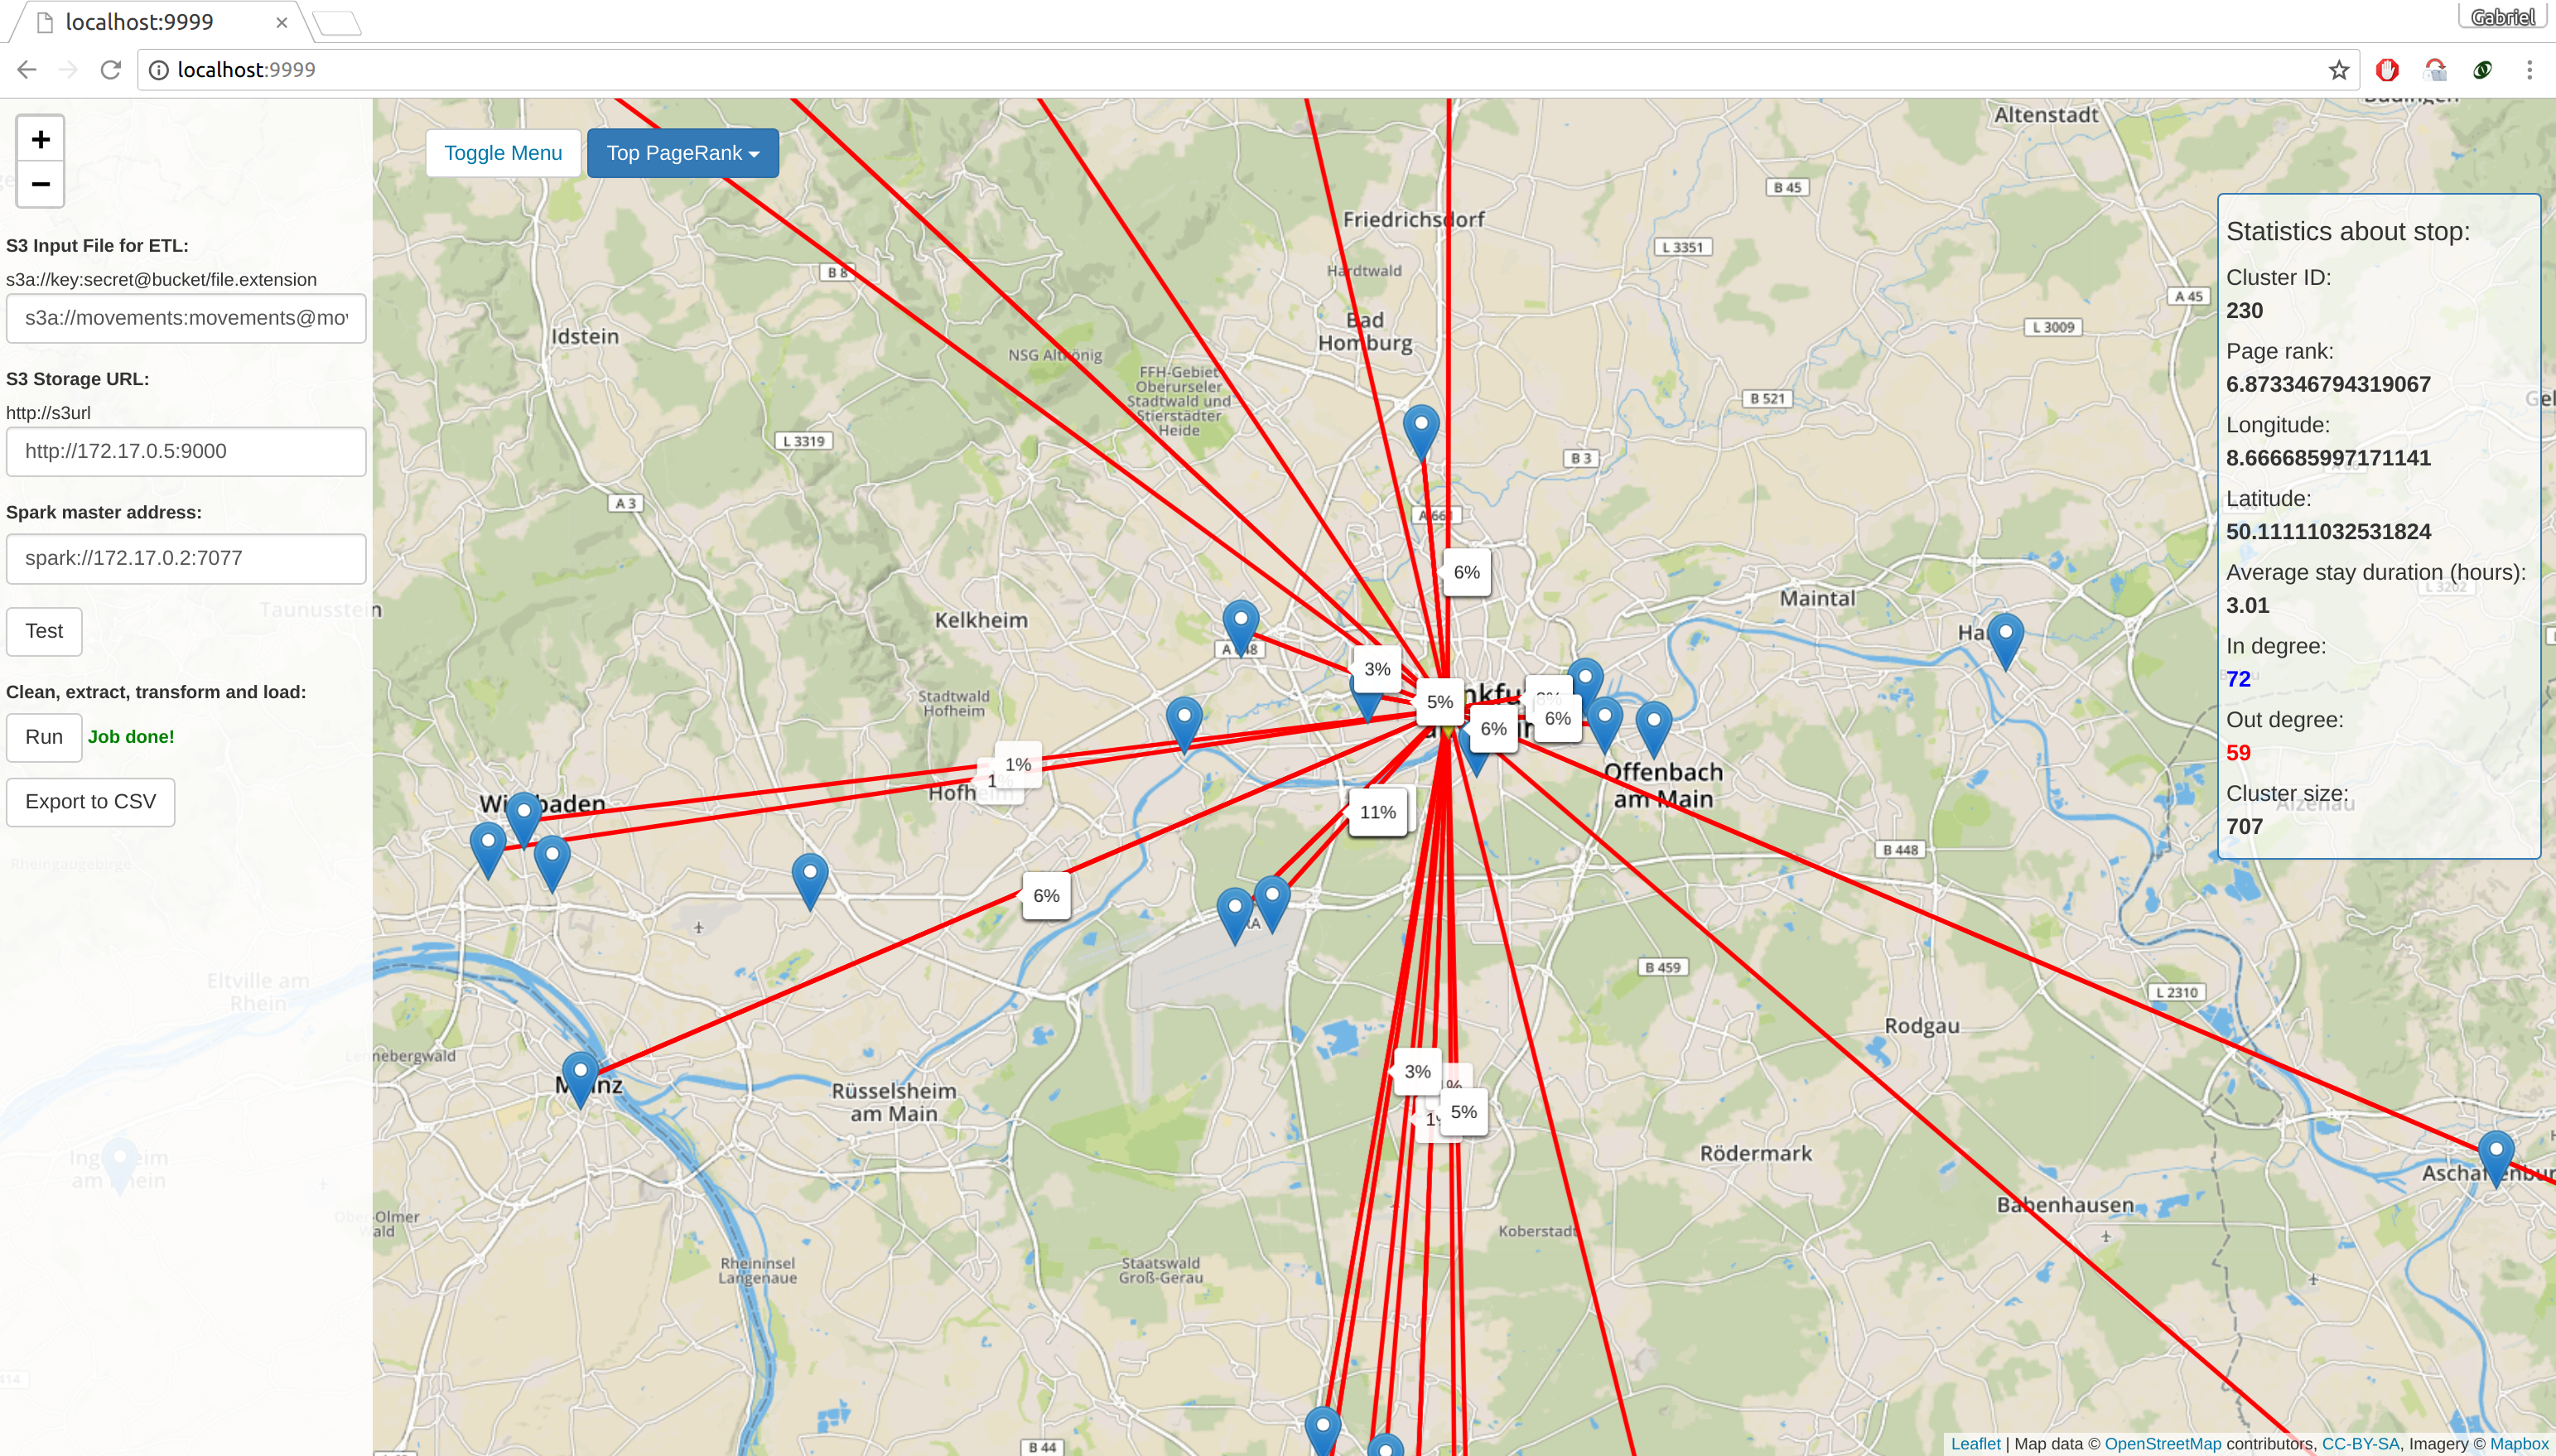
\includegraphics[width=1\textwidth]{images/ui_ger.png}\\
	\caption{ User interface showing clusters and connection from central Frankfurt. }
	\label{fig:0.001_5_gray}
\end{figure}


\section{Graph analysis}
The graph analysis phase was based on the output of clustering phase. Our assumptions were that properties of the graph should help us identify important areas and routes in a city. We chose to analyze clusters in and around Berlin in order to verify our assumptions. Once the graph was created and compared with map of Berlin, we could conclude that the stop algorithm and clustering algorithm worked correctly, as nodes of the graph matched with many well-known areas in the city. 

Now, based on properties extracted from the graph, we tried to understand nature of movements of users and locations of interest. Using properties like in- and out-degrees we could identify key locations that were important as shopping or business areas, residential areas, transport hubs as well due to proximity with airport or Universities.
  
Furthermore, by analyzing the centrality values like betweenness and pagerank we could identify influential nodes that represented key junction in the city transport network. Due to their connectivity and position in the network, they strongly influenced routing decision of users. It was least surprising that some of the most well traveled routes passed through these nodes. 

We could also correctly identify location with high inter-connectivity and verify the results using strongly connected components of the graph. Last but not the least, using trip count measures of the OD matrix, we were able to identify popular routes in Berlin and nearby cities of Spandau and Potsdam.

The results extracted from each of the properties were in sync with each other and also corroborated our assumptions. In this way we can conclude that the results of graph analysis phase could successfully identify key locations and routes in the city and provide a better understanding of user movement patterns.

